% Preamble
\pdfminorversion=4
\documentclass[aspectratio=169]{beamer}
\usepackage{multimedia} % for videos
\usepackage{bm} % for bold math (for tensors)
\usepackage{layout} % put command \layout{} onto an empty frame to see margin lengths
\usepackage{adjustbox}
\usepackage{lipsum}
\usepackage{pdfpages}
\usepackage{hyperref} % for hyperlinks
\usepackage{ulem} % for underline, etc.

% ----- beamer settings -----
% {{{

% define some colors/shades
\definecolor{lightblue}{HTML}{66A3D2}
\definecolor{darkblue}{HTML}{0B61A4}
\definecolor{lightgreen}{HTML}{CFC493}
\definecolor{darkgreen}{HTML}{006747}
\definecolor{lightorange}{HTML}{FF8E0B}
\definecolor{darkorange}{HTML}{D45500}
\definecolor{paleorange}{HTML}{FFDEB3}

% set color for hyperlinks
%\hypersetup{colorlinks, linkcolor=darkgray, citecolor=darkgray, urlcolor=darkgray}
\hypersetup{
    colorlinks=true,
    linkcolor=blue,
    filecolor=magenta,      
    urlcolor=cyan,
    linkbordercolor=darkgreen,
  %  pdfborderstyle={/S/U/W 1},
    }

% set theme
\usetheme{boxes}
\usefonttheme[onlymath]{serif}

% set beamer theme colors, etc.
\setbeamercolor{frametitle}{fg=black}

% customize blocks
\setbeamertemplate{blocks}[rounded][shadow=false]
\setbeamercolor{block title}{fg=white, bg=darkgreen}
\setbeamercolor{block body}{fg=black, bg=lightgreen}

% customize enumerate and item, including color and spacing
\setbeamercolor*{item}{fg=darkgreen}
\setbeamercolor*{enumerate item}{fg=black}
\setbeamercolor*{enumerate subitem}{fg=black}
\setbeamercolor*{enumerate subsubitem}{fg=black}
\setbeamertemplate{itemize subitem}{$-$}
\setlength{\leftmarginii}{10pt}
\newlength\origleftmargini
\setlength\origleftmargini\leftmargini

% customize footer
\setbeamercolor{footline}{fg=gray}
\setbeamertemplate{navigation symbols}{} % get rid of navigation bar

% add page numbers to footer
\makeatletter
\setbeamertemplate{footline}{
    \leavevmode%
    \hbox{%
    \begin{beamercolorbox}[wd=0.5\paperwidth,ht=2.25ex,dp=1ex,left,leftskip=1ex]{}
    \end{beamercolorbox}
    \begin{beamercolorbox}[wd=0.5\paperwidth,ht=2.25ex,dp=1ex,right,rightskip=2ex]{}
      \insertframenumber % page number only
      % \insertframenumber/\inserttotalframenumber % page number/total pages
    \end{beamercolorbox}
    }\vskip0pt
}
\makeatother
% }}}

% ----- tikz ----- (for drawing)
% {{{
\usepackage{tikz}
\usetikzlibrary{shapes,positioning,arrows,backgrounds,fit}
% tikz define invisible: 
% http://tex.stackexchange.com/questions/55806/mindmap-tikzpicture-in-beamer-reveal-step-by-step/55849#55849
\tikzset{
  invisible/.style={opacity=0.2},
  visible on/.style={alt=#1{}{invisible}},
  alt/.code args={<#1>#2#3}{%
    \alt<#1>{\pgfkeysalso{#2}}{\pgfkeysalso{#3}} % \pgfkeysalso doesn't change the path
  },
}

\pgfdeclarelayer{bg}    % declare background layer
\pgfsetlayers{bg,main}  % set the order of the layers (main is the standard layer)

\newcommand{\highlighteq}[2]{ \tikz[baseline]{\node[fill=#1,rounded corners,anchor=base]{$\displaystyle \strut #2$};} }

\tikzset{onslide/.code args={<#1>#2}{%
  \only<#1>{\pgfkeysalso{#2}} % \pgfkeysalso doesn't change the path
}}

% }}}

% --- Notes on options for including movies ---
% {{{

% (1) movie15 package
% \usepackage{movie15}
% \includemovie[text={\includegraphics[width=5cm]{figs/lam_t0.pdf}}]{}{}{figs/lam.avi}
% Comments: 
%   * apparently depreciated (superceded by movie9), but seems to play movies fine
%   * (bad) Puts a pushpin icon over the video
%   * (good) Actually embeds the movie, so don't need to include a separate folder
%   * (bad) Puts black or white bars when playing movie with controls (changes size of
%     the movie to fit the controls into the frame).

% (2) movie9 package
% \usepackage{media9}
% Comments:
%   * Plays using a flash player. Doesn't work on Linux.

% (3) multimedia package
% \usepackage{multimedia}
% \movie[width=5cm, showcontrols]{\includegraphics[width=5cm]{figs/lam_t0.pdf}}{figs/lam.avi}
% Comments:
%   * (good) Seems like the best (but flawed) option for playing a movie in the frame
%   * (bad) Does not embed the movie. Need a separate videos folder.
%   * (bad) Puts black or white bars when playing movie with controls (changes size of
%     the movie to fit the controls into the frame).
%   * (aside) Appears that the backend of the player (same as movie15 pacakge) can be 
%     changed from gstreamer to vlc. Used apt-get install phonon-backend-vlc. Made bars
%     white, not black, which was a marginal improvement.
%     http://tex.stackexchange.com/questions/163089/okular-to-play-embedded-videos-in-beamer

% (4) Hyperlink
% \include{hyperref}
% \href{run:figs/lam.avi}{\includegraphics[width=5cm]{figs/lam_t0.pdf}}
% Comments:
%   * Runs an external viewer (like VLC)
%   * (good) Cross-platform compatible
%   * (bad) Means lots of clicking, and not very easy to move back and forth
%   * (bad) Does not embed the movie. Need a separate videos folder.
%   * (bad) Cannot set up a script to give arguments to external program (e.g. VLC)

% (5) pdfpc
% \href{run:figs/lam.avi?autostart&loop}{\includegraphics[width=5cm]{figs/lam_t0.pdf}}
% Comments:
%   * (neutral) Separate presentation platform. Has nice features.
%   * (bad) Has a slow "pre-rendering" feature.
%   * (bad) All tested videos end up very poor resolution.
%   * (good) Viewer does not re-size videos with ugly controls

% }}}

% ----- tips/tricks & custom definitions ----
% {{{

%% ** block title without a block **
\newcommand{\blocktitle}[1]{
  \begin{tikzpicture}
    \node[ fill, color=darkgreen, text=white, rounded corners, inner sep=4pt,
           align=center, minimum width=4cm, minimum height=\baselineskip
    ] 
    {\large #1\par};
  \end{tikzpicture}
}

% ** columns **
%  \begin{columns}[T]
%    \begin{column}{0.45\textwidth}
%      Column 1: Theory
%    \end{column}
%    \begin{column}{0.45\textwidth}
%      Column 2: Experiment
%    \end{column}
%  \end{columns}

% ** make a figure bigger than the textwidth **
%\makebox[\textwidth][c]{\includegraphics[width=1.0\textwidth]{figs/immersion_precipitation_roll.pdf}}

% ** bulk commenting **
%\iffalse
%\fi

% ** Put citation in bottom middle **
%\begin{tikzpicture}[remember picture, overlay]
%  \node[text width=\textwidth, align=center, anchor=south] at (current page.south) {
%    \scriptsize Lee et al. Adv.~Materials. 29, 1076008 (2017)\par
%  };
%\end{tikzpicture}

% }}}

% custom title page
% {{{
\setbeamerfont{author}{size=\normalsize} % font sizes
\newcommand{\location}[1]{\def\insertlocation{#1}}
\newcommand{\titlecolor}{\color{white}}
\newcommand{\bottomcolor}{\color{white}}
% https://tex.stackexchange.com/questions/350511/latex-beamer-create-own-variable
\newcommand\insertpresenter{}
\newcommand\presenter[1]{\renewcommand\insertpresenter{ \uline{#1}} }

\defbeamertemplate*{title page}{customized}[1][]
{
    \begin{tikzpicture}[remember picture, overlay]

      % background photo
      \node [draw=none, align=center] at (current page.center)
      {
        
\includegraphics[keepaspectratio, width=1.01\paperwidth]{./figs/github_back2.jpeg}
      };

      % BYU logo
      \node [draw=none, align=center, anchor=north west] 
        at ([xshift=-0.05in, yshift=0.05in] current page.north west)
      {
        
\includegraphics[keepaspectratio, width=1.0in]{./figs/USF_logo.png}
      };

     % group logo
      \node [draw=none, align=center, anchor=north east] at (current page.north east)
      {
        
\includegraphics[keepaspectratio, width=2.0in]{./figs/Simmons_logo.png}
      };
  
      % title
      \usebeamercolor{title}
      \node [text width=0.80\paperwidth, align=center, draw=none, fill=black, rounded corners,
             fill opacity=0.5, text opacity=1, inner sep=5pt,
             below = 0.3in of current page.center, anchor=center] 
      {
        {
          \huge \titlecolor{} \inserttitle\par
        }
        \vspace{12pt}
        {
          \Large \bottomcolor{}\insertpresenter \par
        } 
        \vspace{8pt}
        { 
          \bottomcolor{} \insertinstitute \par
        }

      };

      % add date
      \node [draw=none, text width=0.6\paperwidth, anchor=south west] (date)
      at (current page.south west)
      {
        \bottomcolor{}
        \raggedright
        \insertlocation\par
      };

      % add location
      \node [draw=none, above left = 0cm and 0cm of current page.south east, text width=0.6\paperwidth] (date)
      {
        \bottomcolor{}
        \raggedleft
        \insertdate\par
      };

    \end{tikzpicture}
    
}
% }}}

% ----- title/author info -----
\title{A Quick Introduction to Git \& GitHub}
\presenter{Pierre Kawak}
\institute{University of South Florida}
\location{Simmons Lab Group Meeting}
\date{September 8, 2022}

\begin{document}

\begin{frame}[plain]
  % customize title page using the template in the preamble
  \titlepage
\end{frame}

\begin{frame}[c]{GitHub simplifies version control}
% {{{

  % [c] vertically centers your content
  % [t] will top align the content

  \begin{columns}[T]

  \column{0.45\textwidth}

    \centering
%    \vspace{\baselineskip}
    \begin{block}{Git is a god-tier tool}
      \begin{itemize} 
      \item Saves history
      \item Allows collaboration
      \item Tools to search/debug
      \item On the cloud/automatic backups
      \item Move b/w machines
      \item Portable and minimal
    \end{itemize}
    \end{block}

    \begin{block}{What I use it for}
      \begin{itemize} 
      \item Build code
      \item Make presentations
      \item Write papers
    \end{itemize}
    \end{block}

  \column{0.45\textwidth}

    \centering
    \vspace{\baselineskip}
    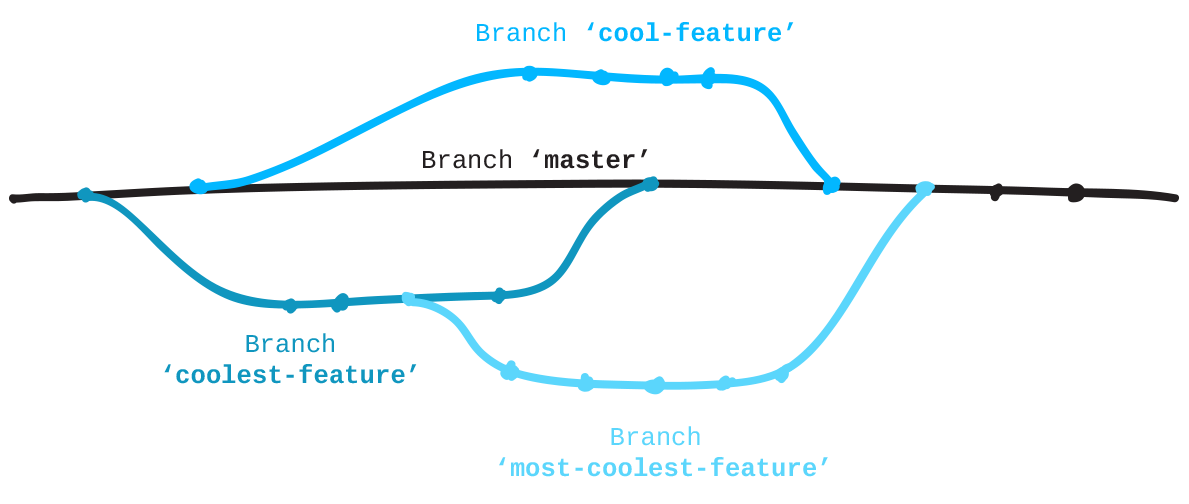
\includegraphics[width=\textwidth]{figs/fig-git_branches.png}

    \vspace{\baselineskip}

    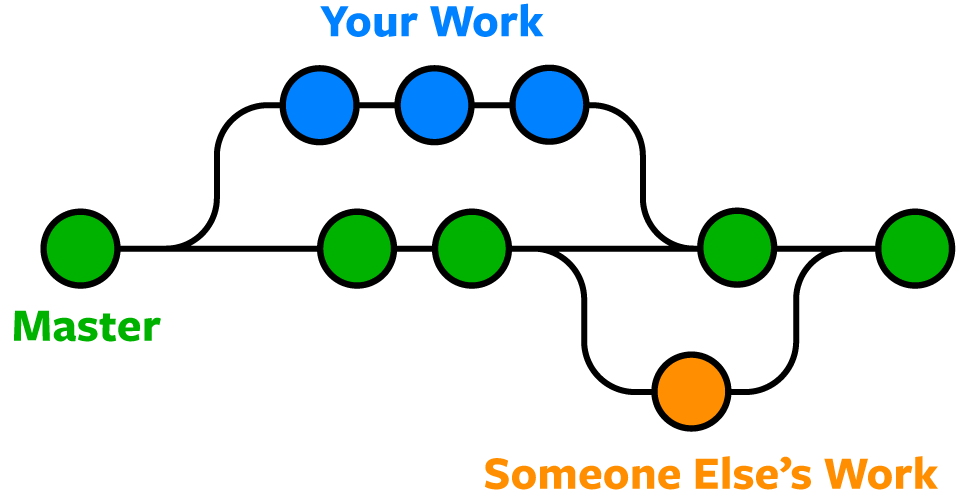
\includegraphics[width=\textwidth]{figs/fig-git_branches_others.png}

  \end{columns}

%% }}}
\end{frame}

\begin{frame}{The basics of Git \& GitHub}
% {{{

    \centering
    \begin{block}{Some tutorial links}
      \begin{itemize} 
      \item Set keys for GitHub to recognize you, i.e. \href{https://docs.github.com/en/authentication/connecting-to-github-with-ssh}{set up ssh keys}
      \item \href{https://docs.github.com/en/get-started/quickstart/create-a-repo}{Creating a repo(sitory)}
      \item Copying work from the cloud to your machine, i.e. \href{https://docs.github.com/en/repositories/creating-and-managing-repositories/cloning-a-repository}{cloning a repo}
      \item How to save your work, i.e. \href{https://github.com/git-guides/git-commit}{commit} \& \href{https://github.com/git-guides/git-push}{push}
    \end{itemize}
    \end{block}

    \vspace{\baselineskip}

    \begin{block}{Let's try this together}
      \begin{itemize} 
      \item Creating a repo and commiting!
      \item Using git bad to debug your code
    \end{itemize}
    \end{block}

%% }}}
\end{frame}

\begin{frame}{The next slides are on my work computer!}
% {{{

  
\includegraphics[width=\textwidth]{figs/oh_no.png}

%% }}}
\end{frame}

\begin{frame}{The basics of Git \& GitHub}
% {{{

    \centering
    \vspace{-0.25\baselineskip}

    \begin{block}{Some tutorial links}
      \begin{itemize} 
      \item Set keys for GitHub to recognize you, i.e. \href{https://docs.github.com/en/authentication/connecting-to-github-with-ssh}{set up ssh keys}
      \item \href{https://docs.github.com/en/get-started/quickstart/create-a-repo}{Creating a repo(sitory)}
      \item Copying work from the cloud to your machine, i.e. \href{https://docs.github.com/en/repositories/creating-and-managing-repositories/cloning-a-repository}{cloning a repo}
      \item How to save your work, i.e. \href{https://github.com/git-guides/git-commit}{commit} \& \href{https://github.com/git-guides/git-push}{push}
    \end{itemize}
    \end{block}

    \begin{block}{Let's try this together}
      \begin{itemize} 
      \item Creating a repo and commiting!
      \item Using git bad to debug your code
      \item \bf{Easy to move between machines}\\git clone git@github.com:/\$\{USER\}/\$\{REPO\}.git
    \end{itemize}
    \end{block}

    \begin{block}{Awesome templates}
      \begin{itemize} 
      \item \href{https://github.com/tree-group-papers/PaperTemplate}{Papers template}
      \item \href{https://github.com/tree-group-other/TalkTemplate}{Talks template}
    \end{itemize}
    \end{block}

%% }}}
\end{frame}

\end{document}

